\documentclass[a4paper,11pt]{ltjsarticle}
% 数式
\usepackage{amsmath,amsfonts}
\usepackage{bm}
% 画像
\usepackage{graphicx}
\usepackage{circuitikz}
\usepackage{amsmath,amssymb}
\usepackage{siunitx}
\usepackage{float}
\usepackage{tikz}
\usepackage{askmaps}
\usepackage{multirow}
\usepackage{bigstrut}
\usepackage{rotating}
\usepackage{listings}
% 数式
\usepackage{physics}
\usepackage{mathtools}
% 画像
\usepackage{subcaption}
% 表
\usepackage{makecell}
% その他
\usepackage{url}
\usepackage{ascmac}
\usepackage{cases}
\usepackage{here}
\usepackage{upgreek}
% 日本語対応
\usepackage{luatexja}
\usepackage{luatexja-fontspec}

\AtBeginDocument{\RenewCommandCopy\qty\SI}


\definecolor{commentgreen}{RGB}{0,200,0}
\definecolor{eminence}{RGB}{120,80,250}
\definecolor{weborange}{RGB}{255,165,0}
\definecolor{frenchplum}{RGB}{10,150,200}
\definecolor{commentgreen}{RGB}{0,200,0}
\definecolor{eminence}{RGB}{120,80,250}
\definecolor{weborange}{RGB}{255,165,0}
\definecolor{frenchplum}{RGB}{10,150,200}

\lstset{
        language = {C},
        basicstyle = \ttfamily\small,
        keywordstyle=\color{eminence}\ttfamily\bfseries,
        commentstyle=\color{commentgreen}\textit,
    identifierstyle=\color{black}\ttfamily,
        xleftmargin=.35in,
        frame=lines,
    showstringspaces=false,
        numbers=left,
        stepnumber = 1,
        breaklines=true,
        numberstyle = \ttfamily\normalsize,
    tabsize=4,  
        emph={int, int8_t, int16_t, int32_t, int64_t, uint8_t, uint16_t, uint32_t, uint64_t, char, double, float, unsigned, void, bool},
        emphstyle={\color{blue}}, 
        morekeywords={>, <, ., ;, +, -, *, /, !, =, ~},
        breakindent = 10pt, 
        framexleftmargin=10mm, 
        columns=fixed,
        basewidth=0.5em,
        }

% 特定のスタイル設定
\lstdefinestyle{customtxt}{
  basicstyle=\ttfamily\footnotesize,
  backgroundcolor=\color{lightgray},
  frame=single,
  breaklines=true,
  columns=fullflexible,
  showspaces=false,
  showstringspaces=false,
  showtabs=false,
  tabsize=4,
}

\newcommand{\fig}[4]{
    \begin{figure}[htbp]
      \centering
      \includegraphics{./image/#1}
      \caption{#2}
      \label{fig:#3}
    \end{figure}
  }
\begin{document}
\title{情報エレクトロニクス実験I\hspace{-1.2pt}I\hspace{-1.2pt}I SQL, データベース}
\author{\empty}
\date{\empty}
\maketitle
\begin{table}[b]
  \centering
  \begin{tabular}{|c|l|}
    \hline
    氏名                   & 古城隆人             \\
    \hline
    学籍番号                 & 22060            \\
    \hline
    組番号                  & 212              \\
    \hline
    所属                   & 情報エレクトロニクス 情報コース \\
    \hline
    \multirow{5}{*}{実験日} & 2025年6月27日       \\
                         & 2025年7月4日        \\
                         & 2025年7月11日       \\
                         & 2025年7月25日       \\
                         & 2025年8月1日        \\
    \hline
    提出日                  & \today           \\
    \hline
  \end{tabular}
\end{table}
\newpage
\clearpage
\section{目的}
データを保存する方法はたくさんあるが，
その中でも情報の分野で複数人で使うことを目的として作られたMySQLを用いて実験を行い，
データベースを使用する方法を学ぶ．
また，データの正規化を行うことにより効率よくデータを保存したり，
属性ごとの種類を見やすくする．この正規化についても手法を学び実際に行うことにより理解を深める．
\section{原理}
\subsection{データベースとはなにか}
データベースとは，データを効率よく保存するものであり，
データの検索や更新，また共有をしやすくするために構造化したものである．
今回の実験ではデータベースを操作するための言語であるSQLを用いる．
データを効率よく保存する方法として，正規化というものがあり，これはデータの冗長性を排除したり，
依存関係ごとのテーブルを作成することによりデータの検索の効率化や保存の効率化を行うものである．
\subsubsection{依存関係とは}
データベースにおける依存関係とは，あるデータが確定した場合，
それに依存しているデータが確定する関係のことである．
例えば学籍番号というデータが任意の一つのものに決まったとき，
その学籍番号が割り当てられている学生についての情報が任意の一つに定まる．このとき，
学籍番号と学生に関するデータは依存関係にあると言える．
この依存関係をデータベースではリレーション(関係)と呼ぶ．
相互にリレーションがあるデータベースのつながりをリレーショナルデータベースと呼ぶ．
\subsubsection{リレーショナルデータベース}
リレーショナルデータベースは，相互につながりがあることが確定されているため，
データの検索を行うときにも依存関係を使用して探すことが出来る．
今回の実験ではこのリレーショナルデータベースを主に用いて正規化を行ったデータについての関係を意識して課題を行っていく．
\subsubsection{そのほかのデータベースの種類}
リレーショナルデータベース以外にも階層型データベースやネットワーク型データベース等の構造がる．
階層型データベースは，関係があまり変わらない場合(リレーションの変更などが行われない場合)によく用いられるものである．
検索の面においても分岐をたどっていく最中に，深いとこまで分岐を探ってから検索を行うことが場合によってはできるため，探索の時間が速くなるなどのメリットがある．
使われているシステムにはファイルシステムなどが挙げられる．
ネットワーク型データベースはそれぞれの情報がノードとして登録され，多対多の関係が構築されている．
使用例としては，予約システムなどが挙げられ，予約の枠に対して複数人の予約がある場合には，
予約する人をそれぞれノードとして登録しておくことにより，予約管理のデータベースでの書き換えはノードとのつながりを書き換えるだけで良くなるため，効率的である．

\subsection{SQLとはなにか}
SQL(Structured Query Language)とは，前述の通りデータベースを操作するための言語である．
データベースにはDBMSというデータベースを管理するシステムが有り，
そこにSQLのコマンドを渡すことでデータベースに変更を加えたり検索を行ったりしている．
コマンドは国際的に標準化されており，様々なデータベースを同じコマンドで操作することができる．
\subsection{MySQL}
MySQLは，データベースシステムの一種である．
データはデータベースの中に複数のテーブルがあり，
テーブルのカラムが最初に設定され，データはカラムの設定に基づいて保存されたり変更されていく．
DBMSではこの設定を見て，例外的な値があった場合にはエラーを出したりし，エラー処理を行う場合もある．
\section{実験}
目標を達成するために行った実験について実験環境と実験の方法について述べる．
\subsection{実験環境}
実験環境を表\ref{tab:environment}に示す．ただし，()の中身は環境等のバージョンを示している．
\begin{table}[H]
  \caption{実装環境}
  \centering
  \begin{tabular}{|c|c|}
    \hline
    OS     & Windows 11 Pro (24H2)        \\
    \hline
    開発環境   & Windows 11 Pro (24H2)        \\
    \hline
    データベース & MySQL (8.4.5)                \\
    \hline
    CPU    & インテル® Core™ i7-11800H プロセッサー \\
    \hline
    メモリ    & 16GB                         \\
    \hline
    SSD    & 512GB                        \\
    \hline
  \end{tabular}
  \label{tab:environment}
\end{table}
\subsection{実験課題}
実験は課題を達成することを目標に行った．
課題は1~3ある．それぞれいかに示す．
\subsection{課題1}
表\ref{tab:rawdata}に示すデータについて正規化を行うものである．
正規化とは，データベースにおいてデータの冗長性を排除して
効率的にデータを保存する手法である．今回は第一正規化,第二正規化,第三正規化について行う．
\begin{table}[htbp]
  \centering
  \caption{学生成績一覧} % 表のキャプション
  \label{tab:rawdata}
  \resizebox{\textwidth}{!}{%
    \begin{tabular}{|c|c|c|c|c|c|l|c|c|c|c|c|} % ← ここが修正ポイント
      \hline
      \textbf{学籍番号}          & \textbf{学生名}           & \textbf{年齢}         & \textbf{性別}        & \textbf{系}                   & \textbf{校舎}         & \textbf{科目名} & \textbf{点数} & \textbf{判定} & \textbf{教員コード} & \textbf{教員名} & \textbf{入力日} \\
      \hline

      % --- 1人目: 山川 一郎 ---
      \multirow{3}{*}{26401} & \multirow{3}{*}{山川 一郎} & \multirow{3}{*}{18} & \multirow{3}{*}{男} & \multirow{3}{*}{都市デザイン系}     & \multirow{3}{*}{C棟} & 国語           & 65          & 可           & G002           & 長松 次郎        & 2025-06-10   \\ \cline{7-12}
                             &                        &                     &                    &                              &                     & 物理           & 42          & 不可          & G001           & 長松 遥         & 2025-06-11   \\ \cline{7-12}
                             &                        &                     &                    &                              &                     & 現代社会         & 79          & 良           & G005           & 高田 真由        & 2025-06-14   \\
      \hline

      % --- 2人目: 谷泉 太郎 ---
      \multirow{3}{*}{26205} & \multirow{3}{*}{谷泉 太郎} & \multirow{3}{*}{19} & \multirow{3}{*}{男} & \multirow{3}{*}{情報エレクトロニクス系} & \multirow{3}{*}{B棟} & 物理           & 76          & 良           & G001           & 長松 遥         & 2025-06-11   \\ \cline{7-12}
                             &                        &                     &                    &                              &                     & 電気工学         & 66          & 可           & E012           & 三浦 裕         & 2025-06-12   \\ \cline{7-12}
                             &                        &                     &                    &                              &                     & 信号処理         & 90          & 優           & E012           & 三浦 裕         & 2025-06-12   \\
      \hline

      % --- 3人目: 海土 花子 ---
      \multirow{3}{*}{26132} & \multirow{3}{*}{海土 花子} & \multirow{3}{*}{20} & \multirow{3}{*}{女} & \multirow{3}{*}{機械ロボティクス系}   & \multirow{3}{*}{A棟} & 物理           & 87          & 優           & G001           & 長松 遥         & 2025-06-10   \\ \cline{7-12}
                             &                        &                     &                    &                              &                     & 機械力学         & 78          & 良           & M301           & 上条 雄三        & 2025-06-11   \\ \cline{7-12}
                             &                        &                     &                    &                              &                     & 計測工学         & 100         & 優           & M553           & 西岡 剛         & 2025-06-12   \\
      \hline
    \end{tabular}
  }
\end{table}
\subsubsection{第一正規化}
第一正規化とは，「テーブルの行と列が交差する特定の1マスに1つの値しか含まない状態にする」ことであるため，
今回の場合は縦のセルについて結合されているところがあるため，セル結合を解除することにより第一正規化が完了する．
\subsubsection{第二正規化}
第二正規化では，主キーという概念を用いてデータの冗長性を排除する．主キーとは，あるものが確定するとそれ以外の情報が確定するものである．
例えば学籍番号から学生に関するデータが確定でき，科目名から科目に関するデータを一つに確定することが出来る．
このような従属している関係を抜き取るのが第二正規化であるため，今回は学籍番号-学生に関するデータ,
科目名-科目に関するデータ,学籍番号と科目名-成績に関するデータとして，3種類の表に分けることが出来る．
\subsubsection{第三正規化}
第二正規化が終わったデータについて，このデータにも冗長性がある．例えば学生に関するデータでは，
校舎に関するデータがあるが，この校舎は学生によって決まっているのではなく，学生が所属している学科によって決まっているので，学籍番号からは間接的なつながりしかない．
そのためこの従属関係を切り離して保存するのが第三正規化である．
そのため，第三正規化では学生,成績,系,校舎,科目,教員,判定,性別をそれぞれ別の表に分けることが出来る．

\subsection{課題2}
課題1で正規化を行ったデータを用いて，SQLを用いてデータベースの作成を行う．
また，SELECT文を用いて入力されたデータがしっかりと格納されているかを確認する．
\subsection{課題3}
課題2で登録したデータに対し，SELECT文を用いてそれぞれの問いに答える．
問については以下に列挙する．
\begin{itemize}
  \item 第 1 正規化したときの表を表示する SQL を定義せよ．
  \item いずれかの科目で判定が優である学生の学籍番号，氏名，系を問い合わせるための SQL
        文を実行し，実行結果を示せ．ただし，条件文は「80 点以上」とせず，「判定が優であ
        る」とすること．
  \item 担当が「高田」または「三浦」の科目を履修している学生について，学生名，科目名，担
        当，判定を問い合わせる SQL 文を実行し，実行結果を示せ． ただし，表示するレコー
        ドは「高田」または「三浦」が担当している科目のもののみでよい．
  \item 科目名に「学」が含まれる科目について，履修している学生名，科目名，点数を問い合
        わせる SQL 文を実行し，実行結果を示せ．
  \item 担当が「三浦」の科目の平均点を問い合わせる SQL 文を実行し，実行結果を示せ．
\end{itemize}
\section{結果}
実験で入力したコマンドとその結果等を示す．
\subsection{課題1}
表\ref{tab:rawdata}のデータを正規化したものについて，第一正規化を表\ref{tab:normarlized1}，
第二正規化したものを表\ref{tab:normalized2_student}と表\ref{tab:normalized2_subject}と表\ref{tab:normalized2_teacher}に示す．
第三正規化したものをについて，学生,成績,系,校舎,科目,教員,判定,性別をそれぞれ
表\ref{tab:normalized3_student}, \ref{tab:normalized3_subject}, \ref{tab:normalized3_department}, \ref{tab:normalized3_campus}, \ref{tab:normalized3_subjects}, \ref{tab:normalized3_teacher}, \ref{tab:normalized3_judgment}
, \ref{tab:normalized3_gender}に示す．
また，第三正規化した結果を ER 図として図\ref{fig:er_diagram}に示す．
\begin{table}[htbp]
  \centering
  \caption{第1正規化}
  \label{tab:normarlized1}
  \resizebox{\textwidth}{!}{%
    \begin{tabular}{|c|c|c|c|c|c|l|c|c|c|c|c|}
      \hline
      \textbf{学籍番号} & \textbf{学生名} & \textbf{年齢} & \textbf{性別} & \textbf{系}  & \textbf{校舎} & \textbf{科目名} & \textbf{点数} & \textbf{判定} & \textbf{教員コード} & \textbf{教員名} & \textbf{入力日} \\
      \hline

      % --- 1人目: 山川 一郎 ---
      \hline
      26401         & 山川 一郎        & 18          & 男           & 都市デザイン系     & C棟          & 国語           & 65          & 可           & G002           & 長松 次郎        & 2025-06-10   \\
      \hline
      26401         & 山川 一郎        & 18          & 男           & 都市デザイン系     & C棟          & 物理           & 42          & 不可          & G001           & 長松 遥         & 2025-06-11   \\
      \hline
      26401         & 山川 一郎        & 18          & 男           & 都市デザイン系     & C棟          & 現代社会         & 79          & 良           & G005           & 高田 真由        & 2025-06-14   \\
      \hline

      % --- 2人目: 谷泉 太郎 ---
      26205         & 谷泉 太郎        & 19          & 男           & 情報エレクトロニクス系 & B棟          & 物理           & 76          & 良           & G001           & 長松 遥         & 2025-06-11   \\
      \hline
      26205         & 谷泉 太郎        & 19          & 男           & 情報エレクトロニクス系 & B棟          & 電気工学         & 66          & 可           & E012           & 三浦 裕         & 2025-06-12   \\
      \hline
      26205         & 谷泉 太郎        & 19          & 男           & 情報エレクトロニクス系 & B棟          & 信号処理         & 90          & 優           & E012           & 三浦 裕         & 2025-06-12   \\
      \hline

      % --- 3人目: 海土 花子 ---
      26132         & 海土 花子        & 20          & 女           & 機械ロボティクス系   & A棟          & 物理           & 87          & 優           & G001           & 長松 遥         & 2025-06-10   \\
      \hline
      26132         & 海土 花子        & 20          & 女           & 機械ロボティクス系   & A棟          & 機械力学         & 78          & 良           & M301           & 上条 雄三        & 2025-06-11   \\
      \hline
      26132         & 海土 花子        & 20          & 女           & 機械ロボティクス系   & A棟          & 計測工学         & 100         & 優           & M553           & 西岡 剛         & 2025-06-12   \\
      \hline
    \end{tabular}
  }
\end{table}
\begin{table}[htbp]
  \centering
  \caption{第2正規化 学生に関するテーブル}
  \label{tab:normalized2_student}
  \begin{tabular}{|c|c|c|c|c|c|}
    \hline
    \textbf{学籍番号} & \textbf{学生名} & \textbf{年齢} & \textbf{性別} & \textbf{系}  & \textbf{校舎} \\
    \hline

    % --- 1人目: 山川 一郎 ---
    26401         & 山川 一郎        & 18          & 男           & 都市デザイン系     & C棟          \\
    \hline

    % --- 2人目: 谷泉 太郎 ---
    26205         & 谷泉 太郎        & 19          & 男           & 情報エレクトロニクス系 & B棟          \\
    \hline

    % --- 3人目: 海土 花子 ---
    26132         & 海土 花子        & 20          & 女           & 機械ロボティクス系   & A棟          \\
    \hline
  \end{tabular}
\end{table}
\begin{table}[htbp]
  \centering
  \caption{第2正規化成績に関するテーブル}
  \label{tab:normalized2_subject}
  \begin{tabular}{|c|c|c|c|c|}
    \hline
    \textbf{学籍番号} & \textbf{科目名} & \textbf{点数} & \textbf{判定} & \textbf{入力日} \\
    \hline

    % --- 1人目: 山川 一郎 ---
    26401         & 国語           & 65          & 可           & 2025-06-10   \\
    \hline
    26401         & 物理           & 42          & 不可          & 2025-06-11   \\
    \hline
    26401         & 現代社会         & 79          & 良           & 2025-06-14   \\
    \hline

    % --- 2人目: 谷泉 太郎 ---
    26205         & 物理           & 76          & 良           & 2025-06-11   \\
    \hline
    26205         & 電気工学         & 66          & 可           & 2025-06-12   \\
    \hline
    26205         & 信号処理         & 90          & 優           & 2025-06-12   \\
    \hline

    % --- 3人目: 海土 花子 ---
    26132         & 物理           & 87          & 優           & 2025-06-10   \\
    \hline
    26132         & 機械力学         & 78          & 良           & 2025-06-11   \\
    \hline
    26132         & 計測工学         & 100         & 優           & 2025-06-12   \\
    \hline
  \end{tabular}
\end{table}
\begin{table}[htbp]
  \centering
  \caption{第2正規化 教師に関するテーブル}
  \label{tab:normalized2_teacher}
  \begin{tabular}{|c|c|c|}
    \hline
    \textbf{科目名} & \textbf{教員コード} & \textbf{教員名} \\
    \hline

    % --- 1人目: 山川 一郎 ---
    国語           & G002           & 長松 次郎        \\ \hline
    物理           & G001           & 長松 遥         \\ \hline
    現代社会         & G005           & 高田 真由        \\
    \hline

    % --- 2人目: 谷泉 太郎 ---
    電気工学         & E012           & 三浦 裕         \\ \hline
    信号処理         & E012           & 三浦 裕         \\
    \hline

    % --- 3人目: 海土 花子 ---
    機械力学         & M301           & 上条 雄三        \\ \hline
    計測工学         & M553           & 西岡 剛         \\
    \hline
  \end{tabular}
\end{table}

\begin{table}[htbp] %学生
  \centering
  \caption{第3正規化 学生に関するデータ}
  \label{tab:normalized3_student}
  \begin{tabular}{|c|c|c|c|c|}
    \hline
    \textbf{学籍番号} & \textbf{学生名} & \textbf{年齢} & \textbf{性別ID} & \textbf{系ID} \\
    \hline

    26401         & 山川 一郎        & 18          & 1             & 3            \\
    \hline

    26205         & 谷泉 太郎        & 19          & 1             & 2            \\
    \hline

    26132         & 海土 花子        & 20          & 2             & 1            \\
    \hline
  \end{tabular}
\end{table}
\begin{table}[htbp] %成績
  \centering
  \caption{第3正規化 成績に関するデータ}
  \label{tab:normalized3_subject}
  \begin{tabular}{|c|c|c|c|}
    \hline
    \textbf{学籍番号} & \textbf{科目ID} & \textbf{点数} & \textbf{入力日} \\
    \hline

    % --- 1人目: 山川 一郎 ---
    26401         & 10003         & 65          & 2025-06-10   \\
    26401         & 10001         & 42          & 2025-06-11   \\
    26401         & 10002         & 79          & 2025-06-14   \\
    \hline

    % --- 2人目: 谷泉 太郎 ---
    26205         & 10001         & 76          & 2025-06-11   \\
    26205         & 10004         & 66          & 2025-06-12   \\
    26205         & 10005         & 90          & 2025-06-12   \\
    \hline

    % --- 3人目: 海土 花子 ---
    26132         & 10001         & 87          & 2025-06-10   \\
    26132         & 10006         & 78          & 2025-06-11   \\
    26132         & 10007         & 100         & 2025-06-12   \\
    \hline
  \end{tabular}
\end{table}

\begin{table}[htbp] %系
  \centering
  \caption{第3正規化 系に関するデータ}
  \label{tab:normalized3_department}
  \begin{tabular}{|c|c|c|}
    \hline
    \textbf{系ID} & \textbf{系}  & \textbf{校舎ID} \\
    \hline

    1            & 機械ロボティクス系   & 30001         \\
    \hline

    2            & 情報エレクトロニクス系 & 30002         \\
    \hline

    3            & 都市デザイン系     & 30003         \\
    \hline
  \end{tabular}
\end{table}

\begin{table}[htbp] %校舎
  \centering
  \caption{第3正規化 校舎に関するデータ}
  \label{tab:normalized3_campus}
  \begin{tabular}{|c|c|}
    \hline
    \textbf{校舎ID} & \textbf{校舎} \\
    \hline

    30001         & A棟          \\
    \hline

    30002         & B棟          \\
    \hline

    30003         & C棟          \\
    \hline
  \end{tabular}
\end{table}

\begin{table}[htbp] %科目
  \centering
  \caption{第3正規化 科目に関するデータ}
  \label{tab:normalized3_subjects}
  \begin{tabular}{|c|c|c|}
    \hline
    \textbf{科目ID} & \textbf{科目名} & \textbf{教員コード} \\
    \hline

    10001         & 物理           & G001           \\ \hline
    10002         & 現代社会         & G005           \\ \hline
    10003         & 国語           & G002           \\ \hline
    10004         & 電気工学         & E012           \\ \hline
    10005         & 信号処理         & E012           \\ \hline
    10006         & 機械力学         & M301           \\ \hline
    10007         & 計測工学         & M553           \\ \hline
  \end{tabular}
\end{table}

\begin{table}[htbp] %教員
  \centering
  \caption{第3正規化 教員に関するデータ}
  \label{tab:normalized3_teacher}
  \begin{tabular}{|c|c|}
    \hline
    \textbf{教員コード} & \textbf{教員名} \\
    \hline

    G002           & 長松 次郎        \\ \hline
    G001           & 長松 遥         \\ \hline
    G005           & 高田 真由        \\ \hline
    E012           & 三浦 裕         \\ \hline
    E012           & 三浦 裕         \\ \hline
    M301           & 上条 雄三        \\ \hline
    M553           & 西岡 剛         \\ \hline
  \end{tabular}
\end{table}

\begin{table}[htbp] %判定
  \centering
  \caption{第3正規化 判定に関するデータ}
  \label{tab:normalized3_judgment}
  \begin{tabular}{|c|c|c|c|}
    \hline
    \textbf{判定ID} & \textbf{下限} & \textbf{上限} & \textbf{判定} \\
    \hline

    1             & 0           & 59          & 不可          \\
    \hline
    2             & 60          & 69          & 可           \\
    \hline
    3             & 70          & 79          & 良           \\
    \hline
    4             & 80          & 100         & 優           \\
    \hline
  \end{tabular}
\end{table}

\begin{table}[htbp] %性別
  \centering
  \caption{第3正規化 性別に関するデータ}
  \label{tab:normalized3_gender}
  \begin{tabular}{|c|c|}
    \hline
    \textbf{性別ID} & \textbf{性別} \\
    \hline

    1             & 男           \\
    \hline

    2             & 女           \\
    \hline
  \end{tabular}
\end{table}
\begin{figure}[htbp]
  \centering
  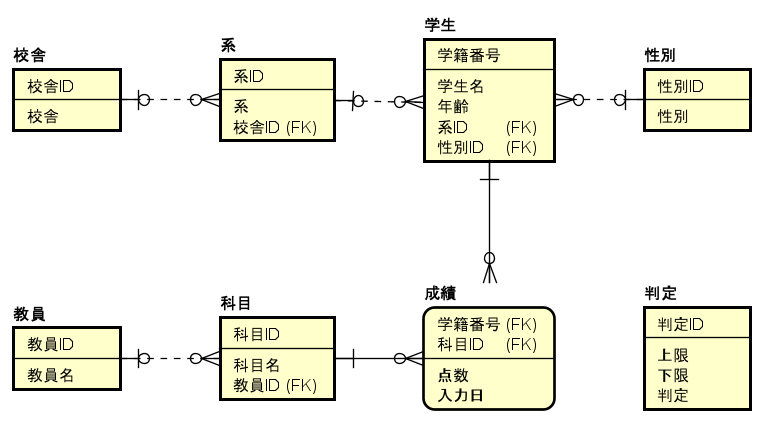
\includegraphics[width=0.8\textwidth]{./image/ER図0.png}
  \caption{ER図}
  \label{fig:er_diagram}
\end{figure}
\newpage
\clearpage
\subsection{課題2}
課題1でER図を作成した際に，各カラムについても設定を行い，そこからSQL文をエクスポートし，テーブルの作成を行あ多後にデータの挿入を行った．
作成したSQL文を\ref{lst:sql}に示す．
実行結果を\ref{lst:sql_result}に示す．
\begin{lstlisting}[caption={SQL文}, label={lst:sql}]
  CREATE DATABASE IF NOT EXISTS kadai;

USE kadai;

DROP TABLE IF EXISTS scores;

DROP TABLE IF EXISTS student;

DROP TABLE IF EXISTS course;

DROP TABLE IF EXISTS subject;

DROP TABLE IF EXISTS place;

DROP TABLE IF EXISTS teacher;

DROP TABLE IF EXISTS gender;

DROP TABLE IF EXISTS result;

CREATE TABLE
    result (
        id INT NOT NULL PRIMARY KEY,
        max INT,
        min INT,
        result VARCHAR(2) NOT NULL
    );

CREATE TABLE
    gender (id INT NOT NULL PRIMARY KEY, gender CHAR(4));

CREATE TABLE
    teacher (
        teacher_id CHAR(4) NOT NULL PRIMARY KEY,
        name VARCHAR(40) NOT NULL
    );

CREATE TABLE
    place (
        id INT NOT NULL PRIMARY KEY,
        place VARCHAR(40) NOT NULL
    );

CREATE TABLE
    subject (
        id INT NOT NULL PRIMARY KEY,
        subject VARCHAR(40) NOT NULL,
        teacher_id CHAR(4) NOT NULL,
        FOREIGN KEY (teacher_id) REFERENCES teacher (teacher_id)
    );

CREATE TABLE
    course (
        id INT NOT NULL PRIMARY KEY,
        course VARCHAR(40) NOT NULL,
        place_id INT,
        FOREIGN KEY (place_id) REFERENCES place (id)
    );

CREATE TABLE
    student (
        code CHAR(5) NOT NULL PRIMARY KEY,
        name VARCHAR(40) NOT NULL,
        age INT,
        icourse_d INT,
        gender_id INT,
        FOREIGN KEY (icourse_d) REFERENCES course (id),
        FOREIGN KEY (gender_id) REFERENCES gender (id)
    );

CREATE TABLE
    scores (
        id INT NOT NULL,
        code CHAR(5) NOT NULL,
        score INT NOT NULL,
        date DATE NOT NULL,
        PRIMARY KEY (id, code),
        FOREIGN KEY (id) REFERENCES subject (id),
        FOREIGN KEY (code) REFERENCES student (code)
    );

INSERT INTO
    result (id, max, min, result)
VALUES
    (1, 59, 0, '不可'),
    (2, 69, 60, '可'),
    (3, 79, 70, '良'),
    (4, 100, 80, '優');

INSERT INTO
    gender (id, gender)
VALUES
    (1, '男'),
    (2, '女');

INSERT INTO
    teacher (teacher_id, name)
VALUES
    ('G002', '長松 次郎'),
    ('G001', '長松 遥'),
    ('G005', '高田 真由'),
    ('E012', '三浦 裕'),
    ('M301', '上条 雄三'),
    ('M553', '西岡 剛');

INSERT INTO
    place (id, place)
VALUES
    (1, 'C棟'),
    (2, 'B棟'),
    (3, 'A棟');

INSERT INTO
    subject (id, subject, teacher_id)
VALUES
    (1, '国語', 'G002'),
    (2, '物理', 'G001'),
    (3, '現代社会', 'G005'),
    (4, '電気工学', 'E012'),
    (5, '信号処理', 'E012'),
    (6, '機械力学', 'M301'),
    (7, '計測工学', 'M553');

INSERT INTO
    course (id, course, place_id)
VALUES
    (1, '都市デザイン系', 1),
    (2, '情報エレクトロニクス系', 2),
    (3, '機械ロボティクス系', 3);

INSERT INTO
    student (code, name, age, icourse_d, gender_id)
VALUES
    ('26401', '山川 一郎', 18, 1, 1),
    ('26205', '谷泉 太郎', 19, 2, 1),
    ('26132', '海土 花子', 20, 3, 2);

INSERT INTO
    scores (id, code, score, date)
VALUES
    (1, '26401', 65, '2025-06-10'),
    (2, '26401', 42, '2025-06-11'),
    (3, '26401', 79, '2025-06-14'),
    (2, '26205', 76, '2025-06-11'),
    (4, '26205', 66, '2025-06-12'),
    (5, '26205', 90, '2025-06-12'),
    (2, '26132', 87, '2025-06-10'),
    (6, '26132', 78, '2025-06-11'),
    (7, '26132', 100, '2025-06-12');

SELECT * FROM result;
SELECT * FROM gender;
SELECT * FROM teacher;
SELECT * FROM place;
SELECT * FROM subject;
SELECT * FROM course;
SELECT * FROM student;
SELECT * FROM scores;
\end{lstlisting}

\begin{lstlisting}[caption={SQL実行結果}, label={lst:sql_result}]
  mysql> source C:\Users\kojor_fyn5sjo\2025\report\informationIII\10w\students.sql
Query OK, 1 row affected, 1 warning (0.08 sec)

Database changed
Query OK, 0 rows affected (0.14 sec)

Query OK, 0 rows affected (0.07 sec)

Query OK, 0 rows affected (0.06 sec)

Query OK, 0 rows affected (0.05 sec)

Query OK, 0 rows affected (0.03 sec)

Query OK, 0 rows affected (0.03 sec)

Query OK, 0 rows affected (0.04 sec)

Query OK, 0 rows affected (0.04 sec)

Query OK, 0 rows affected (0.18 sec)

Query OK, 0 rows affected (0.05 sec)

Query OK, 0 rows affected (0.05 sec)

Query OK, 0 rows affected (0.06 sec)

Query OK, 0 rows affected (0.08 sec)

Query OK, 0 rows affected (0.07 sec)

Query OK, 0 rows affected (0.08 sec)

Query OK, 0 rows affected (0.08 sec)

Query OK, 4 rows affected (0.02 sec)
Records: 4  Duplicates: 0  Warnings: 0

Query OK, 2 rows affected (0.01 sec)
Records: 2  Duplicates: 0  Warnings: 0

Query OK, 6 rows affected (0.02 sec)
Records: 6  Duplicates: 0  Warnings: 0

Query OK, 3 rows affected (0.01 sec)
Records: 3  Duplicates: 0  Warnings: 0

Query OK, 7 rows affected (0.01 sec)
Records: 7  Duplicates: 0  Warnings: 0

Query OK, 3 rows affected (0.01 sec)
Records: 3  Duplicates: 0  Warnings: 0

Query OK, 3 rows affected (0.01 sec)
Records: 3  Duplicates: 0  Warnings: 0

Query OK, 9 rows affected (0.01 sec)
Records: 9  Duplicates: 0  Warnings: 0

+----+------+------+--------+
| id | max  | min  | result |
+----+------+------+--------+
|  1 |   59 |    0 | 不可   |
|  2 |   69 |   60 | 可     |
|  3 |   79 |   70 | 良     |
|  4 |  100 |   80 | 優     |
+----+------+------+--------+
4 rows in set (0.01 sec)

+----+--------+
| id | gender |
+----+--------+
|  1 | 男     |
|  2 | 女     |
+----+--------+
2 rows in set (0.00 sec)

+------------+---------------+
| teacher_id | name          |
+------------+---------------+
| E012       | 三浦 裕       |
| G001       | 長松 遥       |
| G002       | 長松 次郎     |
| G005       | 高田 真由     |
| M301       | 上条 雄三     |
| M553       | 西岡 剛       |
+------------+---------------+
6 rows in set (0.00 sec)

+----+-------+
| id | place |
+----+-------+
|  1 | C棟   |
|  2 | B棟   |
|  3 | A棟   |
+----+-------+
3 rows in set (0.00 sec)

+----+--------------+------------+
| id | subject      | teacher_id |
+----+--------------+------------+
|  1 | 国語         | G002       |
|  2 | 物理         | G001       |
|  3 | 現代社会     | G005       |
|  4 | 電気工学     | E012       |
|  5 | 信号処理     | E012       |
|  6 | 機械力学     | M301       |
|  7 | 計測工学     | M553       |
+----+--------------+------------+
7 rows in set (0.00 sec)

+----+-----------------------------------+----------+
| id | course                            | place_id |
+----+-----------------------------------+----------+
|  1 | 都市デザイン系                    |        1 |
|  2 | 情報エレクトロニクス系            |        2 |
|  3 | 機械ロボティクス系                |        3 |
+----+-----------------------------------+----------+
3 rows in set (0.00 sec)

+-------+---------------+------+-----------+-----------+
| code  | name          | age  | icourse_d | gender_id |
+-------+---------------+------+-----------+-----------+
| 26132 | 海土 花子     |   20 |         3 |         2 |
| 26205 | 谷泉 太郎     |   19 |         2 |         1 |
| 26401 | 山川 一郎     |   18 |         1 |         1 |
+-------+---------------+------+-----------+-----------+
3 rows in set (0.00 sec)

+----+-------+-------+------------+
| id | code  | score | date       |
+----+-------+-------+------------+
|  1 | 26401 |    65 | 2025-06-10 |
|  2 | 26132 |    87 | 2025-06-10 |
|  2 | 26205 |    76 | 2025-06-11 |
|  2 | 26401 |    42 | 2025-06-11 |
|  3 | 26401 |    79 | 2025-06-14 |
|  4 | 26205 |    66 | 2025-06-12 |
|  5 | 26205 |    90 | 2025-06-12 |
|  6 | 26132 |    78 | 2025-06-11 |
|  7 | 26132 |   100 | 2025-06-12 |
+----+-------+-------+------------+
9 rows in set (0.00 sec)
\end{lstlisting}
\subsection{課題3}
それぞれの問いに対するSQL文を以下に示す．
\subsubsection{問1}
inner JOINでテーブルを結合させ，カラムをカラム名にて指定してデータを表示している．
\begin{lstlisting}
  SELECT
    student.code,
    student.name,
    student.age,
    gender.gender,
    course.course,
    place.place,
    subject.subject,
    scores.score,
    result.result,
    teacher.teacher_id,
    teacher.name AS teacher_name,
    scores.date
FROM
    scores
    inner JOIN student ON scores.code = student.code
    inner JOIN course ON student.icourse_d = course.id
    inner JOIN place ON course.place_id = place.id
    inner JOIN gender ON student.gender_id = gender.id
    inner JOIN subject ON scores.id = subject.id
    inner JOIN result ON scores.score between result.min and result.max
    inner JOIN teacher ON subject.teacher_id = teacher.teacher_id
ORDER BY student.code DESC, subject.id ASC;
\end{lstlisting}
\subsubsection{問2}
DISTINCTを入れることにより重複データを消している．基本的にやっていることは問1と変わらないが，WHERE文を用いて成績の判定によりデータの選別を行っている．
\begin{lstlisting}
  SELECT DISTINCT
    student.code,
    student.name,
    course.course
FROM
    scores
    inner JOIN student ON scores.code = student.code
    inner JOIN course ON student.icourse_d = course.id
    inner JOIN place ON course.place_id = place.id
    inner JOIN gender ON student.gender_id = gender.id
    inner JOIN subject ON scores.id = subject.id
    inner JOIN result ON scores.score between result.min and result.max
    inner JOIN teacher ON subject.teacher_id = teacher.teacher_id
WHERE
    result.result = '優';
\end{lstlisting}
\subsubsection{問3}
やっていることは問2とほぼ変わらないが，WHERE文にてワイルドカード検索というもの(LIKE文)を用いている．これは検索に関係のない文字列を一つの文字として扱っているものである．
\begin{lstlisting}
  SELECT
    student.name,
    subject.subject,
    teacher.name AS teacher_name
FROM
    scores
    inner JOIN student ON scores.code = student.code
    inner JOIN course ON student.icourse_d = course.id
    inner JOIN place ON course.place_id = place.id
    inner JOIN gender ON student.gender_id = gender.id
    inner JOIN subject ON scores.id = subject.id
    inner JOIN result ON scores.score between result.min and result.max
    inner JOIN teacher ON subject.teacher_id = teacher.teacher_id
WHERE
    teacher.name LIKE '%高田%'
    OR teacher.name LIKE '%三浦%';
\end{lstlisting}
\subsubsection{問4}
これもやっていることは問3と変わらない．
\begin{lstlisting}
  SELECT
    student.name,
    subject.subject,
    scores.score
FROM
    scores
    inner JOIN student ON scores.code = student.code
    inner JOIN course ON student.icourse_d = course.id
    inner JOIN place ON course.place_id = place.id
    inner JOIN gender ON student.gender_id = gender.id
    inner JOIN subject ON scores.id = subject.id
    inner JOIN result ON scores.score between result.min and result.max
    inner JOIN teacher ON subject.teacher_id = teacher.teacher_id
WHERE
    subject.subject LIKE '%学%';
\end{lstlisting}
\subsubsection{問5}
これはやっていることはほぼ問4と同じだが，SELECT分のカラムの指定のとこで関数を用いている．AVG関数は引数のカラムについての平均をとってくれる関数であり，今回はWHEREにて絞った条件での平均を出している．
\begin{lstlisting}
  SELECT
    AVG(scores.score) AS avg
FROM
    scores
    inner JOIN student ON scores.code = student.code
    inner JOIN course ON student.icourse_d = course.id
    inner JOIN place ON course.place_id = place.id
    inner JOIN gender ON student.gender_id = gender.id
    inner JOIN subject ON scores.id = subject.id
    inner JOIN result ON scores.score between result.min and result.max
    inner JOIN teacher ON subject.teacher_id = teacher.teacher_id
WHERE
    teacher.name LIKE '%三浦%';
\end{lstlisting}
\section{考察}
今回の実験を通して得られた，第三正規までの正規化は大量のデータを保存して検索するときに有用であるという考察について述べる．
\subsection{データの圧縮性}
今回は主にデータベースについて知ること，またデータの冗長性を排除して効率よく保存することについて学んできた．
しかし効率よくの観点で見ると実際には効率が悪く保存されているかもしれない．その理由として，元のデータ性が少ないため冗長性がほぼみられなかった．そのため元のデータ数よりも第三正規化した後のデータの数のほうが多くなってしまい，実際には効率性が落ちてしまっているのではないかと思った．
生徒三件についてのデータのみを保存する場合は，第一正規化までにして保存したほうが圧縮率が保たれているのかもしれない．
しかし，これが生徒200人などの規模になってくると，実際のデータをそのまま保存するよりも統計データのとりやすさ，また検索のしやすさからみて第三正規化までを行ったほうがいいのかもしれない．
\subsection{第三正規化後のデータの保存と運用}
データベースの設計とある程度のサンプルデータについて，手動で入力することにより実験を行ったが，実際にはSQLはプログラムなどから打つことになるだろう．その場合，成績入力受付システム等がSQLを発行することになる．この場合の問題が，複数のテーブルにデータを保存しないといけないという点だ．例えば生徒Aについて今までにない科目を成績に登録した場合書き換えないといけないテーブルは4つある．しかし新しい科目を新設して学生データを入力する際は変更するテーブルが2つである．このように，何を変更するかにより変更するテーブルの数が変わるため，複雑になる．
複雑になることによりプログラムのミス等が増える可能性があるため，そこらへんを意識したデータベースの設計に直したり入力する側に制限を設ける等の対策が必要だと思える．
\subsection{第三正規化による利点}
これまで前項までにてデメリットについて考察をしていたが，メリットについての考察をここではする．
第三正規化まで終わっているデータでは，従属関係が一つしかないため，データとデータのつながりが見えやすい．また，検索したものを表示するときに検索する量をSQLの内部的には減らすことが出来ると思う．その点ではデータの検索が効率的であり，第一正規化に勝るメリットである．しかしこれは保存するデータの量に変わってくるので，今回はその恩恵について感じることが出来なかったが，これが数十万,数百万のデータに対して行われると思うと検索の速度にものすごい影響が出ると思う．






\end{document}